\documentclass[1p]{elsarticle_modified}
%\bibliographystyle{elsarticle-num}

%\usepackage[colorlinks]{hyperref}
%\usepackage{abbrmath_seonhwa} %\Abb, \Ascr, \Acal ,\Abf, \Afrak
\usepackage{amsfonts}
\usepackage{amssymb}
\usepackage{amsmath}
\usepackage{amsthm}
\usepackage{scalefnt}
\usepackage{amsbsy}
\usepackage{kotex}
\usepackage{caption}
\usepackage{subfig}
\usepackage{color}
\usepackage{graphicx}
\usepackage{xcolor} %% white, black, red, green, blue, cyan, magenta, yellow
\usepackage{float}
\usepackage{setspace}
\usepackage{hyperref}

\usepackage{tikz}
\usetikzlibrary{arrows}

\usepackage{multirow}
\usepackage{array} % fixed length table
\usepackage{hhline}

%%%%%%%%%%%%%%%%%%%%%
\makeatletter
\renewcommand*\env@matrix[1][\arraystretch]{%
	\edef\arraystretch{#1}%
	\hskip -\arraycolsep
	\let\@ifnextchar\new@ifnextchar
	\array{*\c@MaxMatrixCols c}}
\makeatother %https://tex.stackexchange.com/questions/14071/how-can-i-increase-the-line-spacing-in-a-matrix
%%%%%%%%%%%%%%%

\usepackage[normalem]{ulem}

\newcommand{\msout}[1]{\ifmmode\text{\sout{\ensuremath{#1}}}\else\sout{#1}\fi}
%SOURCE: \msout is \stkout macro in https://tex.stackexchange.com/questions/20609/strikeout-in-math-mode

\newcommand{\cancel}[1]{
	\ifmmode
	{\color{red}\msout{#1}}
	\else
	{\color{red}\sout{#1}}
	\fi
}

\newcommand{\add}[1]{
	{\color{blue}\uwave{#1}}
}

\newcommand{\replace}[2]{
	\ifmmode
	{\color{red}\msout{#1}}{\color{blue}\uwave{#2}}
	\else
	{\color{red}\sout{#1}}{\color{blue}\uwave{#2}}
	\fi
}

\newcommand{\Sol}{\mathcal{S}} %segment
\newcommand{\D}{D} %diagram
\newcommand{\A}{\mathcal{A}} %arc


%%%%%%%%%%%%%%%%%%%%%%%%%%%%%5 test

\def\sl{\operatorname{\textup{SL}}(2,\Cbb)}
\def\psl{\operatorname{\textup{PSL}}(2,\Cbb)}
\def\quan{\mkern 1mu \triangleright \mkern 1mu}

\theoremstyle{definition}
\newtheorem{thm}{Theorem}[section]
\newtheorem{prop}[thm]{Proposition}
\newtheorem{lem}[thm]{Lemma}
\newtheorem{ques}[thm]{Question}
\newtheorem{cor}[thm]{Corollary}
\newtheorem{defn}[thm]{Definition}
\newtheorem{exam}[thm]{Example}
\newtheorem{rmk}[thm]{Remark}
\newtheorem{alg}[thm]{Algorithm}

\newcommand{\I}{\sqrt{-1}}
\begin{document}

%\begin{frontmatter}
%
%\title{Boundary parabolic representations of knots up to 8 crossings}
%
%%% Group authors per affiliation:
%\author{Yunhi Cho} 
%\address{Department of Mathematics, University of Seoul, Seoul, Korea}
%\ead{yhcho@uos.ac.kr}
%
%
%\author{Seonhwa Kim} %\fnref{s_kim}}
%\address{Center for Geometry and Physics, Institute for Basic Science, Pohang, 37673, Korea}
%\ead{ryeona17@ibs.re.kr}
%
%\author{Hyuk Kim}
%\address{Department of Mathematical Sciences, Seoul National University, Seoul 08826, Korea}
%\ead{hyukkim@snu.ac.kr}
%
%\author{Seokbeom Yoon}
%\address{Department of Mathematical Sciences, Seoul National University, Seoul, 08826,  Korea}
%\ead{sbyoon15@snu.ac.kr}
%
%\begin{abstract}
%We find all boundary parabolic representation of knots up to 8 crossings.
%
%\end{abstract}
%\begin{keyword}
%    \MSC[2010] 57M25 
%\end{keyword}
%
%\end{frontmatter}

%\linenumbers
%\tableofcontents
%
\newcommand\colored[1]{\textcolor{white}{\rule[-0.35ex]{0.8em}{1.4ex}}\kern-0.8em\color{red} #1}%
%\newcommand\colored[1]{\textcolor{white}{ #1}\kern-2.17ex	\textcolor{white}{ #1}\kern-1.81ex	\textcolor{white}{ #1}\kern-2.15ex\color{red}#1	}

{\Large $\underline{12a_{0816}~(K12a_{0816})}$}

\setlength{\tabcolsep}{10pt}
\renewcommand{\arraystretch}{1.6}
\vspace{1cm}\begin{tabular}{m{100pt}>{\centering\arraybackslash}m{274pt}}
\multirow{5}{120pt}{
	\centering
	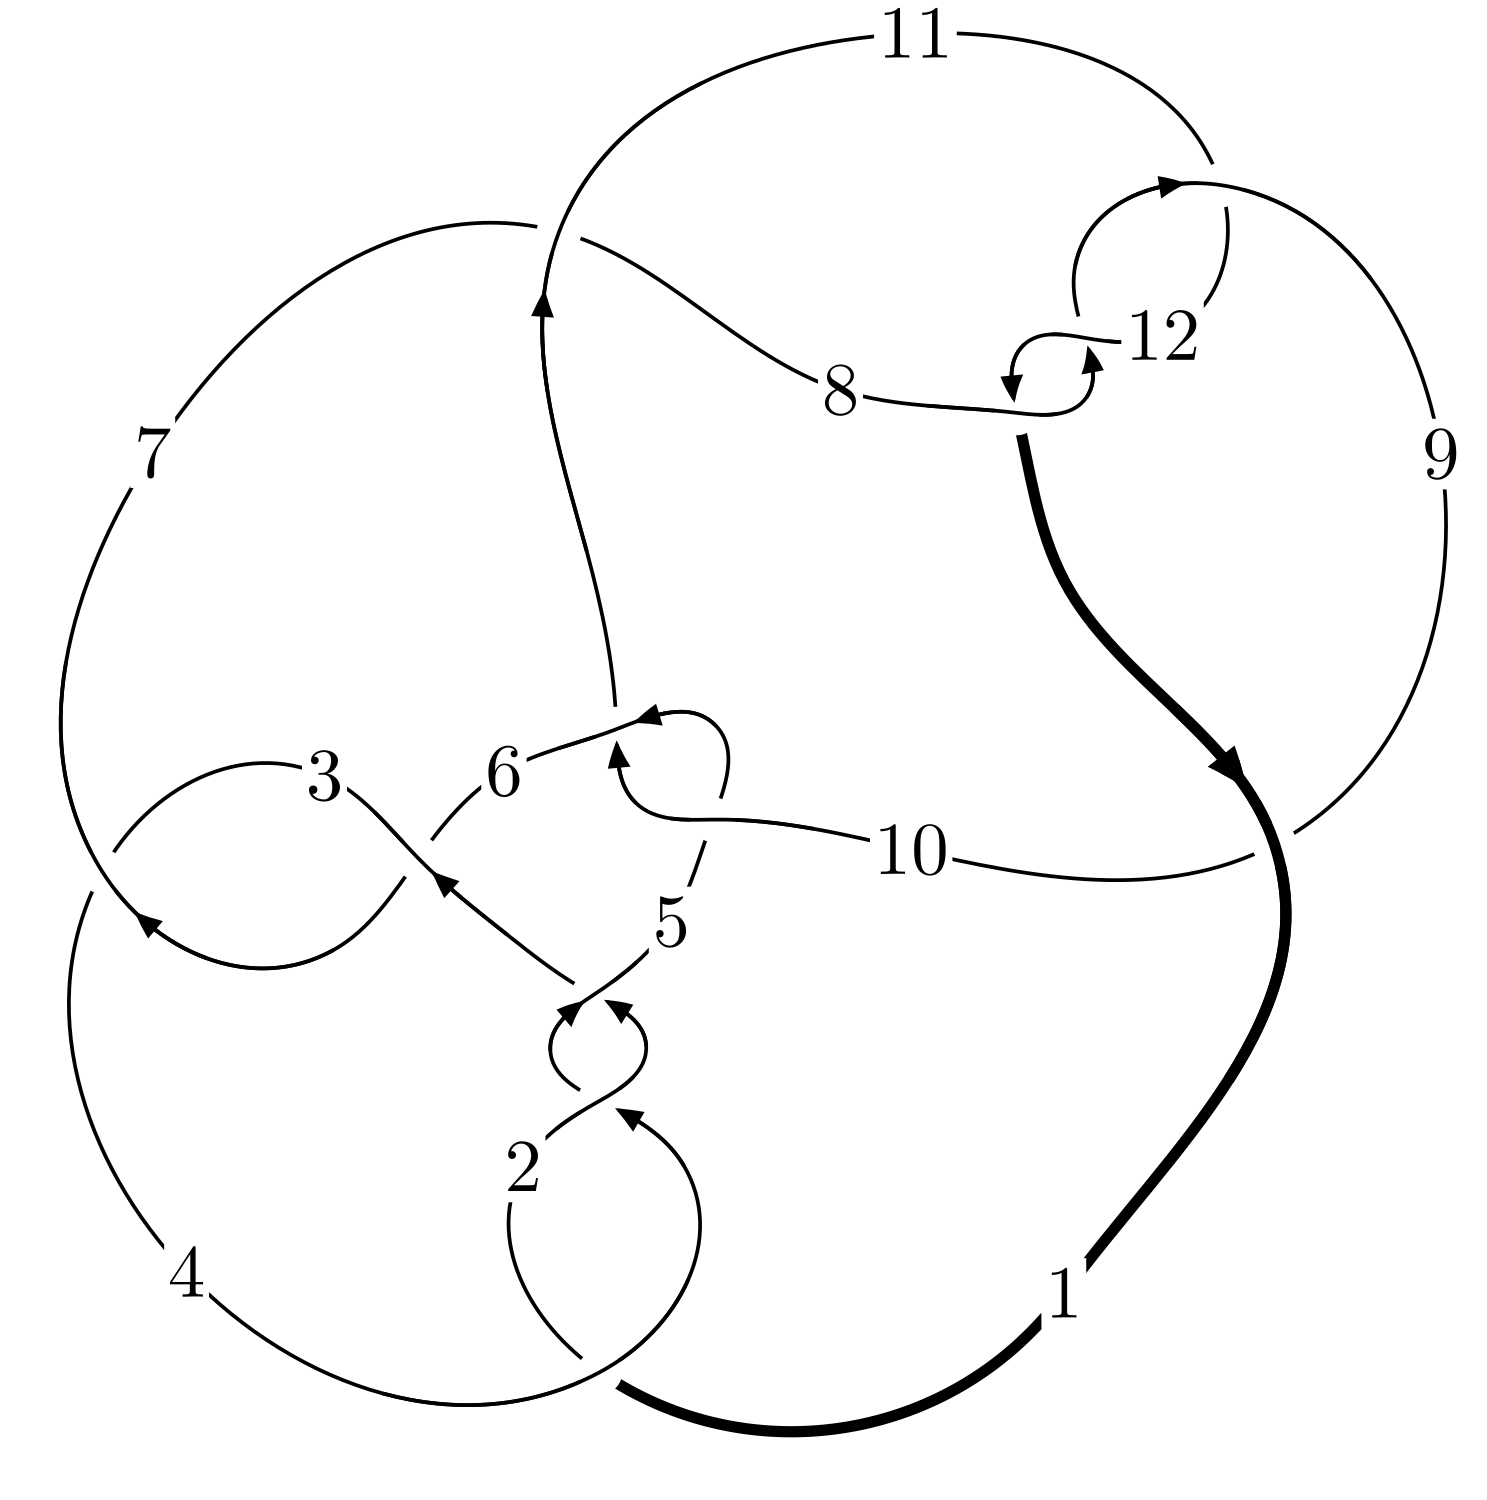
\includegraphics[width=112pt]{../../../GIT/diagram.site/Diagrams/png/1617_12a_0816.png}\\
\ \ \ A knot diagram\footnotemark}&
\allowdisplaybreaks
\textbf{Linearized knot diagam} \\
\cline{2-2}
 &
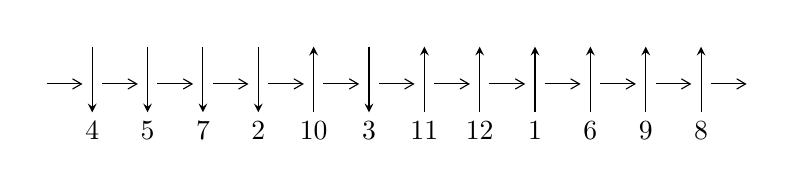
\begin{tikzpicture}[x=20pt, y=17pt]
	% nodes
	\node (C0) at (0, 0) {};
	\node (C1) at (1, 0) {};
	\node (C1U) at (1, +1) {};
	\node (C1D) at (1, -1) {4};

	\node (C2) at (2, 0) {};
	\node (C2U) at (2, +1) {};
	\node (C2D) at (2, -1) {5};

	\node (C3) at (3, 0) {};
	\node (C3U) at (3, +1) {};
	\node (C3D) at (3, -1) {7};

	\node (C4) at (4, 0) {};
	\node (C4U) at (4, +1) {};
	\node (C4D) at (4, -1) {2};

	\node (C5) at (5, 0) {};
	\node (C5U) at (5, +1) {};
	\node (C5D) at (5, -1) {10};

	\node (C6) at (6, 0) {};
	\node (C6U) at (6, +1) {};
	\node (C6D) at (6, -1) {3};

	\node (C7) at (7, 0) {};
	\node (C7U) at (7, +1) {};
	\node (C7D) at (7, -1) {11};

	\node (C8) at (8, 0) {};
	\node (C8U) at (8, +1) {};
	\node (C8D) at (8, -1) {12};

	\node (C9) at (9, 0) {};
	\node (C9U) at (9, +1) {};
	\node (C9D) at (9, -1) {1};

	\node (C10) at (10, 0) {};
	\node (C10U) at (10, +1) {};
	\node (C10D) at (10, -1) {6};

	\node (C11) at (11, 0) {};
	\node (C11U) at (11, +1) {};
	\node (C11D) at (11, -1) {9};

	\node (C12) at (12, 0) {};
	\node (C12U) at (12, +1) {};
	\node (C12D) at (12, -1) {8};
	\node (C13) at (13, 0) {};

	% arrows
	\draw[->,>={angle 60}]
	(C0) edge (C1) (C1) edge (C2) (C2) edge (C3) (C3) edge (C4) (C4) edge (C5) (C5) edge (C6) (C6) edge (C7) (C7) edge (C8) (C8) edge (C9) (C9) edge (C10) (C10) edge (C11) (C11) edge (C12) (C12) edge (C13) ;	\draw[->,>=stealth]
	(C1U) edge (C1D) (C2U) edge (C2D) (C3U) edge (C3D) (C4U) edge (C4D) (C5D) edge (C5U) (C6U) edge (C6D) (C7D) edge (C7U) (C8D) edge (C8U) (C9D) edge (C9U) (C10D) edge (C10U) (C11D) edge (C11U) (C12D) edge (C12U) ;
	\end{tikzpicture} \\
\hhline{~~} \\& 
\textbf{Solving Sequence} \\ \cline{2-2} 
 &
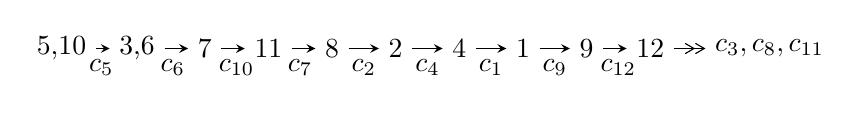
\begin{tikzpicture}[x=23pt, y=7pt]
	% node
	\node (A0) at (-1/8, 0) {5,10};
	\node (A1) at (17/16, 0) {3,6};
	\node (A2) at (17/8, 0) {7};
	\node (A3) at (25/8, 0) {11};
	\node (A4) at (33/8, 0) {8};
	\node (A5) at (41/8, 0) {2};
	\node (A6) at (49/8, 0) {4};
	\node (A7) at (57/8, 0) {1};
	\node (A8) at (65/8, 0) {9};
	\node (A9) at (73/8, 0) {12};
	\node (C1) at (1/2, -1) {$c_{5}$};
	\node (C2) at (13/8, -1) {$c_{6}$};
	\node (C3) at (21/8, -1) {$c_{10}$};
	\node (C4) at (29/8, -1) {$c_{7}$};
	\node (C5) at (37/8, -1) {$c_{2}$};
	\node (C6) at (45/8, -1) {$c_{4}$};
	\node (C7) at (53/8, -1) {$c_{1}$};
	\node (C8) at (61/8, -1) {$c_{9}$};
	\node (C9) at (69/8, -1) {$c_{12}$};
	\node (A10) at (11, 0) {$c_{3},c_{8},c_{11}$};

	% edge
	\draw[->,>=stealth]	
	(A0) edge (A1) (A1) edge (A2) (A2) edge (A3) (A3) edge (A4) (A4) edge (A5) (A5) edge (A6) (A6) edge (A7) (A7) edge (A8) (A8) edge (A9) ;
	\draw[->>,>={angle 60}]	
	(A9) edge (A10);
\end{tikzpicture} \\ 

\end{tabular} \\

\footnotetext{
The image of knot diagram is generated by the software ``\textbf{Draw programme}" developed by Andrew Bartholomew(\url{http://www.layer8.co.uk/maths/draw/index.htm\#Running-draw}), where we modified some parts for our purpose(\url{https://github.com/CATsTAILs/LinksPainter}).
}\phantom \\ \newline 
\centering \textbf{Ideals for irreducible components\footnotemark of $X_{\text{par}}$} 
 
\begin{align*}
I^u_{1}&=\langle 
3.88375\times10^{234} u^{85}-1.46902\times10^{234} u^{84}+\cdots+2.70951\times10^{236} b+2.78190\times10^{236},\\
\phantom{I^u_{1}}&\phantom{= \langle  }1.64525\times10^{236} u^{85}+2.08852\times10^{236} u^{84}+\cdots+5.41901\times10^{236} a+7.89723\times10^{237},\\
\phantom{I^u_{1}}&\phantom{= \langle  }u^{86}+2 u^{85}+\cdots+352 u+64\rangle \\
I^u_{2}&=\langle 
b+1,\;u^5-4 u^3+u^2+a+4 u-3,\;u^6+u^5-3 u^4-2 u^3+2 u^2- u-1\rangle \\
\\
I^v_{1}&=\langle 
a,\;8 v^5+21 v^4+63 v^3+21 v^2+503 b- v-817,\;v^6+3 v^5+v^4-18 v^3-7 v^2+1\rangle \\
\end{align*}
\raggedright * 3 irreducible components of $\dim_{\mathbb{C}}=0$, with total 98 representations.\\
\footnotetext{All coefficients of polynomials are rational numbers. But the coefficients are sometimes approximated in decimal forms when there is not enough margin.}
\newpage
\renewcommand{\arraystretch}{1}
\centering \section*{I. $I^u_{1}= \langle 3.88\times10^{234} u^{85}-1.47\times10^{234} u^{84}+\cdots+2.71\times10^{236} b+2.78\times10^{236},\;1.65\times10^{236} u^{85}+2.09\times10^{236} u^{84}+\cdots+5.42\times10^{236} a+7.90\times10^{237},\;u^{86}+2 u^{85}+\cdots+352 u+64 \rangle$}
\flushleft \textbf{(i) Arc colorings}\\
\begin{tabular}{m{7pt} m{180pt} m{7pt} m{180pt} }
\flushright $a_{5}=$&$\begin{pmatrix}1\\0\end{pmatrix}$ \\
\flushright $a_{10}=$&$\begin{pmatrix}0\\u\end{pmatrix}$ \\
\flushright $a_{3}=$&$\begin{pmatrix}-0.303607 u^{85}-0.385406 u^{84}+\cdots-98.1776 u-14.5732\\-0.0143338 u^{85}+0.00542171 u^{84}+\cdots-2.27870 u-1.02672\end{pmatrix}$ \\
\flushright $a_{6}=$&$\begin{pmatrix}1\\- u^2\end{pmatrix}$ \\
\flushright $a_{7}=$&$\begin{pmatrix}-0.400196 u^{85}-0.562734 u^{84}+\cdots-159.471 u-37.7347\\0.0373459 u^{85}+0.124701 u^{84}+\cdots+33.4026 u+11.9056\end{pmatrix}$ \\
\flushright $a_{11}=$&$\begin{pmatrix}u\\- u^3+u\end{pmatrix}$ \\
\flushright $a_{8}=$&$\begin{pmatrix}-0.364855 u^{85}-0.475874 u^{84}+\cdots-132.797 u-29.2352\\0.103811 u^{85}+0.242890 u^{84}+\cdots+68.0341 u+21.4406\end{pmatrix}$ \\
\flushright $a_{2}=$&$\begin{pmatrix}-0.317940 u^{85}-0.379984 u^{84}+\cdots-100.456 u-15.5999\\-0.0143338 u^{85}+0.00542171 u^{84}+\cdots-2.27870 u-1.02672\end{pmatrix}$ \\
\flushright $a_{4}=$&$\begin{pmatrix}-0.000379134 u^{85}-0.00662213 u^{84}+\cdots+10.0057 u+7.46172\\0.0314098 u^{85}-0.0261001 u^{84}+\cdots-6.20145 u-6.59007\end{pmatrix}$ \\
\flushright $a_{1}=$&$\begin{pmatrix}-0.313635 u^{85}-0.494466 u^{84}+\cdots-134.831 u-34.4302\\0.0865603 u^{85}+0.0682676 u^{84}+\cdots+24.6403 u+3.30443\end{pmatrix}$ \\
\flushright $a_{9}=$&$\begin{pmatrix}-0.428449 u^{85}-0.506093 u^{84}+\cdots-128.967 u-23.4151\\-0.112532 u^{85}-0.102360 u^{84}+\cdots-14.4207 u-1.77881\end{pmatrix}$ \\
\flushright $a_{12}=$&$\begin{pmatrix}-0.518000 u^{85}-0.878705 u^{84}+\cdots-263.329 u-71.7071\\-0.388762 u^{85}-0.550043 u^{84}+\cdots-149.561 u-34.9025\end{pmatrix}$\\&\end{tabular}
\flushleft \textbf{(ii) Obstruction class $= -1$}\\~\\
\flushleft \textbf{(iii) Cusp Shapes $= -1.25246 u^{85}-1.96111 u^{84}+\cdots-563.188 u-165.262$}\\~\\
\newpage\renewcommand{\arraystretch}{1}
\flushleft \textbf{(iv) u-Polynomials at the component}\newline \\
\begin{tabular}{m{50pt}|m{274pt}}
Crossings & \hspace{64pt}u-Polynomials at each crossing \\
\hline $$\begin{aligned}c_{1},c_{2},c_{4}\end{aligned}$$&$\begin{aligned}
&u^{86}-10 u^{85}+\cdots+18 u+1
\end{aligned}$\\
\hline $$\begin{aligned}c_{3},c_{6}\end{aligned}$$&$\begin{aligned}
&u^{86}+4 u^{85}+\cdots-1152 u^2+64
\end{aligned}$\\
\hline $$\begin{aligned}c_{5},c_{10}\end{aligned}$$&$\begin{aligned}
&u^{86}+2 u^{85}+\cdots+352 u+64
\end{aligned}$\\
\hline $$\begin{aligned}c_{7},c_{9}\end{aligned}$$&$\begin{aligned}
&u^{86}-4 u^{85}+\cdots-13134 u+977
\end{aligned}$\\
\hline $$\begin{aligned}c_{8},c_{11},c_{12}\end{aligned}$$&$\begin{aligned}
&u^{86}+4 u^{85}+\cdots-8 u+1
\end{aligned}$\\
\hline
\end{tabular}\\~\\
\newpage\renewcommand{\arraystretch}{1}
\flushleft \textbf{(v) Riley Polynomials at the component}\newline \\
\begin{tabular}{m{50pt}|m{274pt}}
Crossings & \hspace{64pt}Riley Polynomials at each crossing \\
\hline $$\begin{aligned}c_{1},c_{2},c_{4}\end{aligned}$$&$\begin{aligned}
&y^{86}-82 y^{85}+\cdots-478 y+1
\end{aligned}$\\
\hline $$\begin{aligned}c_{3},c_{6}\end{aligned}$$&$\begin{aligned}
&y^{86}-48 y^{85}+\cdots-147456 y+4096
\end{aligned}$\\
\hline $$\begin{aligned}c_{5},c_{10}\end{aligned}$$&$\begin{aligned}
&y^{86}-42 y^{85}+\cdots-107520 y+4096
\end{aligned}$\\
\hline $$\begin{aligned}c_{7},c_{9}\end{aligned}$$&$\begin{aligned}
&y^{86}-56 y^{85}+\cdots-14579676 y+954529
\end{aligned}$\\
\hline $$\begin{aligned}c_{8},c_{11},c_{12}\end{aligned}$$&$\begin{aligned}
&y^{86}+72 y^{85}+\cdots-20 y+1
\end{aligned}$\\
\hline
\end{tabular}\\~\\
\newpage\flushleft \textbf{(vi) Complex Volumes and Cusp Shapes}
$$\begin{array}{c|c|c}  
\text{Solutions to }I^u_{1}& \I (\text{vol} + \sqrt{-1}CS) & \text{Cusp shape}\\
 \hline 
\begin{aligned}
u &= \phantom{-}0.552054 + 0.828557 I \\
a &= \phantom{-}0.192966 - 0.000278 I \\
b &= \phantom{-}1.55396 + 0.16056 I\end{aligned}
 & -13.69310 - 2.82580 I & \phantom{-0.000000 } 0 \\ \hline\begin{aligned}
u &= \phantom{-}0.552054 - 0.828557 I \\
a &= \phantom{-}0.192966 + 0.000278 I \\
b &= \phantom{-}1.55396 - 0.16056 I\end{aligned}
 & -13.69310 + 2.82580 I & \phantom{-0.000000 } 0 \\ \hline\begin{aligned}
u &= \phantom{-}0.712992 + 0.675491 I \\
a &= \phantom{-}0.581320 + 0.515681 I \\
b &= -0.631213 - 0.658080 I\end{aligned}
 & -6.37937 + 0.07950 I & \phantom{-0.000000 } 0 \\ \hline\begin{aligned}
u &= \phantom{-}0.712992 - 0.675491 I \\
a &= \phantom{-}0.581320 - 0.515681 I \\
b &= -0.631213 + 0.658080 I\end{aligned}
 & -6.37937 - 0.07950 I & \phantom{-0.000000 } 0 \\ \hline\begin{aligned}
u &= \phantom{-}0.293714 + 0.923956 I \\
a &= \phantom{-}0.598122 + 0.230114 I \\
b &= -0.220725 - 0.596939 I\end{aligned}
 & \phantom{-}1.77443 - 1.89708 I & \phantom{-0.000000 } 0 \\ \hline\begin{aligned}
u &= \phantom{-}0.293714 - 0.923956 I \\
a &= \phantom{-}0.598122 - 0.230114 I \\
b &= -0.220725 + 0.596939 I\end{aligned}
 & \phantom{-}1.77443 + 1.89708 I & \phantom{-0.000000 } 0 \\ \hline\begin{aligned}
u &= -0.399332 + 0.964359 I \\
a &= \phantom{-}0.562555 - 0.274132 I \\
b &= -0.274017 + 0.680285 I\end{aligned}
 & -2.56815 + 5.72788 I & \phantom{-0.000000 } 0 \\ \hline\begin{aligned}
u &= -0.399332 - 0.964359 I \\
a &= \phantom{-}0.562555 + 0.274132 I \\
b &= -0.274017 - 0.680285 I\end{aligned}
 & -2.56815 - 5.72788 I & \phantom{-0.000000 } 0 \\ \hline\begin{aligned}
u &= -0.814919 + 0.658478 I \\
a &= -0.82638 + 1.33174 I \\
b &= -1.383480 - 0.068743 I\end{aligned}
 & -8.14347 - 2.53737 I & \phantom{-0.000000 } 0 \\ \hline\begin{aligned}
u &= -0.814919 - 0.658478 I \\
a &= -0.82638 - 1.33174 I \\
b &= -1.383480 + 0.068743 I\end{aligned}
 & -8.14347 + 2.53737 I & \phantom{-0.000000 } 0\\
 \hline 
 \end{array}$$\newpage$$\begin{array}{c|c|c}  
\text{Solutions to }I^u_{1}& \I (\text{vol} + \sqrt{-1}CS) & \text{Cusp shape}\\
 \hline 
\begin{aligned}
u &= -0.983266 + 0.394126 I \\
a &= \phantom{-}0.04078 + 1.47966 I \\
b &= -0.260699 - 0.690733 I\end{aligned}
 & \phantom{-}0.29357 - 3.54409 I & \phantom{-0.000000 } 0 \\ \hline\begin{aligned}
u &= -0.983266 - 0.394126 I \\
a &= \phantom{-}0.04078 - 1.47966 I \\
b &= -0.260699 + 0.690733 I\end{aligned}
 & \phantom{-}0.29357 + 3.54409 I & \phantom{-0.000000 } 0 \\ \hline\begin{aligned}
u &= -0.225473 + 0.906689 I \\
a &= \phantom{-}0.191216 - 0.000872 I \\
b &= \phantom{-}1.48450 - 0.07065 I\end{aligned}
 & -8.06829 + 1.47587 I & -6.04730 + 0. I\phantom{ +0.000000I} \\ \hline\begin{aligned}
u &= -0.225473 - 0.906689 I \\
a &= \phantom{-}0.191216 + 0.000872 I \\
b &= \phantom{-}1.48450 + 0.07065 I\end{aligned}
 & -8.06829 - 1.47587 I & -6.04730 + 0. I\phantom{ +0.000000I} \\ \hline\begin{aligned}
u &= -1.049590 + 0.241828 I \\
a &= \phantom{-}0.357510 - 0.885888 I \\
b &= -1.048150 + 0.593109 I\end{aligned}
 & -0.89394 + 2.01684 I & \phantom{-0.000000 } 0 \\ \hline\begin{aligned}
u &= -1.049590 - 0.241828 I \\
a &= \phantom{-}0.357510 + 0.885888 I \\
b &= -1.048150 - 0.593109 I\end{aligned}
 & -0.89394 - 2.01684 I & \phantom{-0.000000 } 0 \\ \hline\begin{aligned}
u &= -0.130183 + 0.912720 I \\
a &= \phantom{-}0.615451 - 0.146529 I \\
b &= -0.106806 + 0.503836 I\end{aligned}
 & -1.74508 - 1.81197 I & \phantom{-0.000000 } 0 \\ \hline\begin{aligned}
u &= -0.130183 - 0.912720 I \\
a &= \phantom{-}0.615451 + 0.146529 I \\
b &= -0.106806 - 0.503836 I\end{aligned}
 & -1.74508 + 1.81197 I & \phantom{-0.000000 } 0 \\ \hline\begin{aligned}
u &= \phantom{-}0.909805 + 0.583851 I \\
a &= -0.30401 - 1.55635 I \\
b &= -0.426541 + 0.738548 I\end{aligned}
 & -5.77290 + 4.80475 I & \phantom{-0.000000 } 0 \\ \hline\begin{aligned}
u &= \phantom{-}0.909805 - 0.583851 I \\
a &= -0.30401 + 1.55635 I \\
b &= -0.426541 - 0.738548 I\end{aligned}
 & -5.77290 - 4.80475 I & \phantom{-0.000000 } 0\\
 \hline 
 \end{array}$$\newpage$$\begin{array}{c|c|c}  
\text{Solutions to }I^u_{1}& \I (\text{vol} + \sqrt{-1}CS) & \text{Cusp shape}\\
 \hline 
\begin{aligned}
u &= \phantom{-}1.048040 + 0.370428 I \\
a &= \phantom{-}0.390246 + 0.782737 I \\
b &= -0.981638 - 0.659900 I\end{aligned}
 & \phantom{-}2.46498 + 1.91776 I & \phantom{-0.000000 } 0 \\ \hline\begin{aligned}
u &= \phantom{-}1.048040 - 0.370428 I \\
a &= \phantom{-}0.390246 - 0.782737 I \\
b &= -0.981638 + 0.659900 I\end{aligned}
 & \phantom{-}2.46498 - 1.91776 I & \phantom{-0.000000 } 0 \\ \hline\begin{aligned}
u &= \phantom{-}0.771535 + 0.431699 I \\
a &= -0.47760 - 1.71983 I \\
b &= -1.262540 + 0.145425 I\end{aligned}
 & -2.36374 + 1.81286 I & \phantom{-0.000000 } 0. - 3.83527 I \\ \hline\begin{aligned}
u &= \phantom{-}0.771535 - 0.431699 I \\
a &= -0.47760 + 1.71983 I \\
b &= -1.262540 - 0.145425 I\end{aligned}
 & -2.36374 - 1.81286 I & \phantom{-0.000000 -}0. + 3.83527 I \\ \hline\begin{aligned}
u &= \phantom{-}0.852981 + 0.159244 I \\
a &= \phantom{-}0.58828 - 1.49094 I \\
b &= -0.159548 + 0.473962 I\end{aligned}
 & \phantom{-}1.120900 + 0.300961 I & \phantom{-}6.91660 - 0.58498 I \\ \hline\begin{aligned}
u &= \phantom{-}0.852981 - 0.159244 I \\
a &= \phantom{-}0.58828 + 1.49094 I \\
b &= -0.159548 - 0.473962 I\end{aligned}
 & \phantom{-}1.120900 - 0.300961 I & \phantom{-}6.91660 + 0.58498 I \\ \hline\begin{aligned}
u &= \phantom{-}1.059140 + 0.410939 I \\
a &= -0.287658 - 1.211040 I \\
b &= -1.376810 + 0.289151 I\end{aligned}
 & -1.68586 + 0.96431 I & \phantom{-0.000000 } 0 \\ \hline\begin{aligned}
u &= \phantom{-}1.059140 - 0.410939 I \\
a &= -0.287658 + 1.211040 I \\
b &= -1.376810 - 0.289151 I\end{aligned}
 & -1.68586 - 0.96431 I & \phantom{-0.000000 } 0 \\ \hline\begin{aligned}
u &= -1.060240 + 0.459416 I \\
a &= \phantom{-}0.391196 - 0.717519 I \\
b &= -0.943184 + 0.714225 I\end{aligned}
 & -1.95224 - 5.90463 I & \phantom{-0.000000 } 0 \\ \hline\begin{aligned}
u &= -1.060240 - 0.459416 I \\
a &= \phantom{-}0.391196 + 0.717519 I \\
b &= -0.943184 - 0.714225 I\end{aligned}
 & -1.95224 + 5.90463 I & \phantom{-0.000000 } 0\\
 \hline 
 \end{array}$$\newpage$$\begin{array}{c|c|c}  
\text{Solutions to }I^u_{1}& \I (\text{vol} + \sqrt{-1}CS) & \text{Cusp shape}\\
 \hline 
\begin{aligned}
u &= \phantom{-}0.438702 + 0.719830 I \\
a &= -1.86531 - 1.41789 I \\
b &= -1.244600 - 0.118813 I\end{aligned}
 & -5.13889 - 4.02609 I & -2.76635 + 0.76522 I \\ \hline\begin{aligned}
u &= \phantom{-}0.438702 - 0.719830 I \\
a &= -1.86531 + 1.41789 I \\
b &= -1.244600 + 0.118813 I\end{aligned}
 & -5.13889 + 4.02609 I & -2.76635 - 0.76522 I \\ \hline\begin{aligned}
u &= -1.081380 + 0.516007 I \\
a &= -0.405516 + 1.145080 I \\
b &= -1.43564 - 0.25261 I\end{aligned}
 & \phantom{-}1.40001 - 4.97319 I & \phantom{-0.000000 } 0 \\ \hline\begin{aligned}
u &= -1.081380 - 0.516007 I \\
a &= -0.405516 - 1.145080 I \\
b &= -1.43564 + 0.25261 I\end{aligned}
 & \phantom{-}1.40001 + 4.97319 I & \phantom{-0.000000 } 0 \\ \hline\begin{aligned}
u &= -1.136010 + 0.403070 I \\
a &= -1.18436 - 1.39457 I \\
b &= \phantom{-}1.41697 + 0.15814 I\end{aligned}
 & -9.55306 + 0.49039 I & \phantom{-0.000000 } 0 \\ \hline\begin{aligned}
u &= -1.136010 - 0.403070 I \\
a &= -1.18436 + 1.39457 I \\
b &= \phantom{-}1.41697 - 0.15814 I\end{aligned}
 & -9.55306 - 0.49039 I & \phantom{-0.000000 } 0 \\ \hline\begin{aligned}
u &= -0.562219 + 0.524976 I \\
a &= \phantom{-}0.716658 - 0.329576 I \\
b &= \phantom{-}0.182504 + 0.015855 I\end{aligned}
 & -3.19093 - 1.95911 I & \phantom{-}3.32674 + 3.69322 I \\ \hline\begin{aligned}
u &= -0.562219 - 0.524976 I \\
a &= \phantom{-}0.716658 + 0.329576 I \\
b &= \phantom{-}0.182504 - 0.015855 I\end{aligned}
 & -3.19093 + 1.95911 I & \phantom{-}3.32674 - 3.69322 I \\ \hline\begin{aligned}
u &= \phantom{-}1.092220 + 0.579762 I \\
a &= -0.466720 - 1.099830 I \\
b &= -1.46979 + 0.22913 I\end{aligned}
 & -3.18556 + 9.02341 I & \phantom{-0.000000 } 0 \\ \hline\begin{aligned}
u &= \phantom{-}1.092220 - 0.579762 I \\
a &= -0.466720 + 1.099830 I \\
b &= -1.46979 - 0.22913 I\end{aligned}
 & -3.18556 - 9.02341 I & \phantom{-0.000000 } 0\\
 \hline 
 \end{array}$$\newpage$$\begin{array}{c|c|c}  
\text{Solutions to }I^u_{1}& \I (\text{vol} + \sqrt{-1}CS) & \text{Cusp shape}\\
 \hline 
\begin{aligned}
u &= -1.187690 + 0.506855 I \\
a &= -0.111325 + 1.217970 I \\
b &= -0.237680 - 0.887129 I\end{aligned}
 & \phantom{-}1.53780 - 3.15145 I & \phantom{-0.000000 } 0 \\ \hline\begin{aligned}
u &= -1.187690 - 0.506855 I \\
a &= -0.111325 - 1.217970 I \\
b &= -0.237680 + 0.887129 I\end{aligned}
 & \phantom{-}1.53780 + 3.15145 I & \phantom{-0.000000 } 0 \\ \hline\begin{aligned}
u &= \phantom{-}1.291170 + 0.123828 I \\
a &= \phantom{-}0.278328 + 0.884185 I \\
b &= \phantom{-}0.269267 - 0.656632 I\end{aligned}
 & \phantom{-}3.52569 - 2.53556 I & \phantom{-0.000000 } 0 \\ \hline\begin{aligned}
u &= \phantom{-}1.291170 - 0.123828 I \\
a &= \phantom{-}0.278328 - 0.884185 I \\
b &= \phantom{-}0.269267 + 0.656632 I\end{aligned}
 & \phantom{-}3.52569 + 2.53556 I & \phantom{-0.000000 } 0 \\ \hline\begin{aligned}
u &= -0.657648 + 0.222079 I \\
a &= \phantom{-}0.190415 + 0.000646 I \\
b &= \phantom{-}1.68329 - 0.04881 I\end{aligned}
 & -11.53680 - 3.32788 I & \phantom{-}1.60100 + 7.68257 I \\ \hline\begin{aligned}
u &= -0.657648 - 0.222079 I \\
a &= \phantom{-}0.190415 - 0.000646 I \\
b &= \phantom{-}1.68329 + 0.04881 I\end{aligned}
 & -11.53680 + 3.32788 I & \phantom{-}1.60100 - 7.68257 I \\ \hline\begin{aligned}
u &= \phantom{-}1.127830 + 0.663427 I \\
a &= -0.35766 + 1.65601 I \\
b &= \phantom{-}1.47079 - 0.27396 I\end{aligned}
 & -11.8702 + 8.4794 I & \phantom{-0.000000 } 0 \\ \hline\begin{aligned}
u &= \phantom{-}1.127830 - 0.663427 I \\
a &= -0.35766 - 1.65601 I \\
b &= \phantom{-}1.47079 + 0.27396 I\end{aligned}
 & -11.8702 - 8.4794 I & \phantom{-0.000000 } 0 \\ \hline\begin{aligned}
u &= -1.294930 + 0.226061 I \\
a &= \phantom{-}0.289669 - 0.819710 I \\
b &= \phantom{-}0.347991 + 0.605697 I\end{aligned}
 & \phantom{-}7.12157 - 1.76447 I & \phantom{-0.000000 } 0 \\ \hline\begin{aligned}
u &= -1.294930 - 0.226061 I \\
a &= \phantom{-}0.289669 + 0.819710 I \\
b &= \phantom{-}0.347991 - 0.605697 I\end{aligned}
 & \phantom{-}7.12157 + 1.76447 I & \phantom{-0.000000 } 0\\
 \hline 
 \end{array}$$\newpage$$\begin{array}{c|c|c}  
\text{Solutions to }I^u_{1}& \I (\text{vol} + \sqrt{-1}CS) & \text{Cusp shape}\\
 \hline 
\begin{aligned}
u &= \phantom{-}1.231000 + 0.473921 I \\
a &= -0.82743 + 1.23132 I \\
b &= \phantom{-}1.381250 - 0.202296 I\end{aligned}
 & -3.88741 + 2.87017 I & \phantom{-0.000000 } 0 \\ \hline\begin{aligned}
u &= \phantom{-}1.231000 - 0.473921 I \\
a &= -0.82743 - 1.23132 I \\
b &= \phantom{-}1.381250 + 0.202296 I\end{aligned}
 & -3.88741 - 2.87017 I & \phantom{-0.000000 } 0 \\ \hline\begin{aligned}
u &= -0.432450 + 1.250560 I \\
a &= \phantom{-}0.193237 - 0.006450 I \\
b &= \phantom{-}1.367100 - 0.183599 I\end{aligned}
 & -6.49234 + 0.65249 I & \phantom{-0.000000 } 0 \\ \hline\begin{aligned}
u &= -0.432450 - 1.250560 I \\
a &= \phantom{-}0.193237 + 0.006450 I \\
b &= \phantom{-}1.367100 + 0.183599 I\end{aligned}
 & -6.49234 - 0.65249 I & \phantom{-0.000000 } 0 \\ \hline\begin{aligned}
u &= -0.353875 + 0.574365 I \\
a &= -2.39311 + 2.12630 I \\
b &= -1.150500 + 0.085662 I\end{aligned}
 & -0.680663 + 0.581964 I & \phantom{-}4.76633 + 3.68087 I \\ \hline\begin{aligned}
u &= -0.353875 - 0.574365 I \\
a &= -2.39311 - 2.12630 I \\
b &= -1.150500 - 0.085662 I\end{aligned}
 & -0.680663 - 0.581964 I & \phantom{-}4.76633 - 3.68087 I \\ \hline\begin{aligned}
u &= \phantom{-}1.189690 + 0.590585 I \\
a &= -0.192525 - 1.202200 I \\
b &= -0.293585 + 0.928049 I\end{aligned}
 & \phantom{-}4.52893 + 7.39783 I & \phantom{-0.000000 } 0 \\ \hline\begin{aligned}
u &= \phantom{-}1.189690 - 0.590585 I \\
a &= -0.192525 + 1.202200 I \\
b &= -0.293585 - 0.928049 I\end{aligned}
 & \phantom{-}4.52893 - 7.39783 I & \phantom{-0.000000 } 0 \\ \hline\begin{aligned}
u &= \phantom{-}1.294060 + 0.316520 I \\
a &= \phantom{-}0.291115 + 0.764351 I \\
b &= \phantom{-}0.414957 - 0.554533 I\end{aligned}
 & \phantom{-}2.91745 + 6.05254 I & \phantom{-0.000000 } 0 \\ \hline\begin{aligned}
u &= \phantom{-}1.294060 - 0.316520 I \\
a &= \phantom{-}0.291115 - 0.764351 I \\
b &= \phantom{-}0.414957 + 0.554533 I\end{aligned}
 & \phantom{-}2.91745 - 6.05254 I & \phantom{-0.000000 } 0\\
 \hline 
 \end{array}$$\newpage$$\begin{array}{c|c|c}  
\text{Solutions to }I^u_{1}& \I (\text{vol} + \sqrt{-1}CS) & \text{Cusp shape}\\
 \hline 
\begin{aligned}
u &= \phantom{-}0.537174 + 1.231980 I \\
a &= \phantom{-}0.196295 + 0.005454 I \\
b &= \phantom{-}1.389820 + 0.235157 I\end{aligned}
 & -3.37770 - 4.95391 I & \phantom{-0.000000 } 0 \\ \hline\begin{aligned}
u &= \phantom{-}0.537174 - 1.231980 I \\
a &= \phantom{-}0.196295 - 0.005454 I \\
b &= \phantom{-}1.389820 - 0.235157 I\end{aligned}
 & -3.37770 + 4.95391 I & \phantom{-0.000000 } 0 \\ \hline\begin{aligned}
u &= -1.181470 + 0.644258 I \\
a &= -0.244491 + 1.194170 I \\
b &= -0.333360 - 0.947743 I\end{aligned}
 & -0.12892 - 11.58520 I & \phantom{-0.000000 } 0 \\ \hline\begin{aligned}
u &= -1.181470 - 0.644258 I \\
a &= -0.244491 - 1.194170 I \\
b &= -0.333360 + 0.947743 I\end{aligned}
 & -0.12892 + 11.58520 I & \phantom{-0.000000 } 0 \\ \hline\begin{aligned}
u &= -0.602863 + 1.211500 I \\
a &= \phantom{-}0.197803 - 0.003918 I \\
b &= \phantom{-}1.41379 - 0.26593 I\end{aligned}
 & -7.97081 + 9.17889 I & \phantom{-0.000000 } 0 \\ \hline\begin{aligned}
u &= -0.602863 - 1.211500 I \\
a &= \phantom{-}0.197803 + 0.003918 I \\
b &= \phantom{-}1.41379 + 0.26593 I\end{aligned}
 & -7.97081 - 9.17889 I & \phantom{-0.000000 } 0 \\ \hline\begin{aligned}
u &= -1.232100 + 0.594842 I \\
a &= -0.51016 - 1.34439 I \\
b &= \phantom{-}1.40089 + 0.26628 I\end{aligned}
 & -4.99770 - 7.01531 I & \phantom{-0.000000 } 0 \\ \hline\begin{aligned}
u &= -1.232100 - 0.594842 I \\
a &= -0.51016 + 1.34439 I \\
b &= \phantom{-}1.40089 - 0.26628 I\end{aligned}
 & -4.99770 + 7.01531 I & \phantom{-0.000000 } 0 \\ \hline\begin{aligned}
u &= -0.560073 + 0.243224 I \\
a &= \phantom{-}1.11682 + 2.93594 I \\
b &= -0.400437 - 0.305942 I\end{aligned}
 & -3.84146 + 2.44487 I & \phantom{-}2.67833 + 5.70811 I \\ \hline\begin{aligned}
u &= -0.560073 - 0.243224 I \\
a &= \phantom{-}1.11682 - 2.93594 I \\
b &= -0.400437 + 0.305942 I\end{aligned}
 & -3.84146 - 2.44487 I & \phantom{-}2.67833 - 5.70811 I\\
 \hline 
 \end{array}$$\newpage$$\begin{array}{c|c|c}  
\text{Solutions to }I^u_{1}& \I (\text{vol} + \sqrt{-1}CS) & \text{Cusp shape}\\
 \hline 
\begin{aligned}
u &= -0.447171 + 0.368366 I \\
a &= \phantom{-}0.977140 - 0.529183 I \\
b &= -0.649137 + 0.321962 I\end{aligned}
 & -1.244520 + 0.136004 I & -5.67462 + 0.66860 I \\ \hline\begin{aligned}
u &= -0.447171 - 0.368366 I \\
a &= \phantom{-}0.977140 + 0.529183 I \\
b &= -0.649137 - 0.321962 I\end{aligned}
 & -1.244520 - 0.136004 I & -5.67462 - 0.66860 I \\ \hline\begin{aligned}
u &= \phantom{-}0.559835\phantom{ +0.000000I} \\
a &= \phantom{-}0.190472\phantom{ +0.000000I} \\
b &= \phantom{-}1.67112\phantom{ +0.000000I}\end{aligned}
 & -7.43832\phantom{ +0.000000I} & \phantom{-}13.1970\phantom{ +0.000000I} \\ \hline\begin{aligned}
u &= -1.26876 + 0.73301 I \\
a &= -0.171599 - 1.310850 I \\
b &= \phantom{-}1.42110 + 0.35592 I\end{aligned}
 & -3.74537 - 7.60591 I & \phantom{-0.000000 } 0 \\ \hline\begin{aligned}
u &= -1.26876 - 0.73301 I \\
a &= -0.171599 + 1.310850 I \\
b &= \phantom{-}1.42110 - 0.35592 I\end{aligned}
 & -3.74537 + 7.60591 I & \phantom{-0.000000 } 0 \\ \hline\begin{aligned}
u &= -1.22662 + 0.81031 I \\
a &= -0.010802 - 1.395770 I \\
b &= \phantom{-}1.47568 + 0.37982 I\end{aligned}
 & -5.9049 - 16.3706 I & \phantom{-0.000000 } 0 \\ \hline\begin{aligned}
u &= -1.22662 - 0.81031 I \\
a &= -0.010802 + 1.395770 I \\
b &= \phantom{-}1.47568 - 0.37982 I\end{aligned}
 & -5.9049 + 16.3706 I & \phantom{-0.000000 } 0 \\ \hline\begin{aligned}
u &= \phantom{-}1.24904 + 0.78295 I \\
a &= -0.069120 + 1.354280 I \\
b &= \phantom{-}1.45236 - 0.37556 I\end{aligned}
 & -1.03547 + 12.08560 I & \phantom{-0.000000 } 0 \\ \hline\begin{aligned}
u &= \phantom{-}1.24904 - 0.78295 I \\
a &= -0.069120 - 1.354280 I \\
b &= \phantom{-}1.45236 + 0.37556 I\end{aligned}
 & -1.03547 - 12.08560 I & \phantom{-0.000000 } 0 \\ \hline\begin{aligned}
u &= \phantom{-}0.099100 + 0.510038 I \\
a &= -5.06181 - 1.25504 I \\
b &= -1.001060 - 0.128912 I\end{aligned}
 & -4.35085 + 2.48127 I & -12.9227 - 14.9608 I\\
 \hline 
 \end{array}$$\newpage$$\begin{array}{c|c|c}  
\text{Solutions to }I^u_{1}& \I (\text{vol} + \sqrt{-1}CS) & \text{Cusp shape}\\
 \hline 
\begin{aligned}
u &= \phantom{-}0.099100 - 0.510038 I \\
a &= -5.06181 + 1.25504 I \\
b &= -1.001060 + 0.128912 I\end{aligned}
 & -4.35085 - 2.48127 I & -12.9227 + 14.9608 I \\ \hline\begin{aligned}
u &= \phantom{-}0.446361\phantom{ +0.000000I} \\
a &= \phantom{-}1.34862\phantom{ +0.000000I} \\
b &= -0.0485703\phantom{ +0.000000I}\end{aligned}
 & \phantom{-}0.791292\phantom{ +0.000000I} & \phantom{-}12.9620\phantom{ +0.000000I} \\ \hline\begin{aligned}
u &= -0.390544\phantom{ +0.000000I} \\
a &= \phantom{-}2.53371\phantom{ +0.000000I} \\
b &= -0.859860\phantom{ +0.000000I}\end{aligned}
 & -1.16619\phantom{ +0.000000I} & -12.5130\phantom{ +0.000000I} \\ \hline\begin{aligned}
u &= \phantom{-}1.68218 + 0.12717 I \\
a &= -0.651799 + 0.146716 I \\
b &= \phantom{-}1.190290 - 0.040584 I\end{aligned}
 & \phantom{-}1.47173 + 4.79342 I & \phantom{-0.000000 } 0 \\ \hline\begin{aligned}
u &= \phantom{-}1.68218 - 0.12717 I \\
a &= -0.651799 - 0.146716 I \\
b &= \phantom{-}1.190290 + 0.040584 I\end{aligned}
 & \phantom{-}1.47173 - 4.79342 I & \phantom{-0.000000 } 0 \\ \hline\begin{aligned}
u &= -1.70399\phantom{ +0.000000I} \\
a &= -0.648277\phantom{ +0.000000I} \\
b &= \phantom{-}1.18657\phantom{ +0.000000I}\end{aligned}
 & \phantom{-}5.42800\phantom{ +0.000000I} & \phantom{-0.000000 } 0\\
 \hline 
 \end{array}$$\newpage\newpage\renewcommand{\arraystretch}{1}
\centering \section*{II. $I^u_{2}= \langle b+1,\;u^5-4 u^3+u^2+a+4 u-3,\;u^6+u^5-3 u^4-2 u^3+2 u^2- u-1 \rangle$}
\flushleft \textbf{(i) Arc colorings}\\
\begin{tabular}{m{7pt} m{180pt} m{7pt} m{180pt} }
\flushright $a_{5}=$&$\begin{pmatrix}1\\0\end{pmatrix}$ \\
\flushright $a_{10}=$&$\begin{pmatrix}0\\u\end{pmatrix}$ \\
\flushright $a_{3}=$&$\begin{pmatrix}- u^5+4 u^3- u^2-4 u+3\\-1\end{pmatrix}$ \\
\flushright $a_{6}=$&$\begin{pmatrix}1\\- u^2\end{pmatrix}$ \\
\flushright $a_{7}=$&$\begin{pmatrix}1\\- u^2\end{pmatrix}$ \\
\flushright $a_{11}=$&$\begin{pmatrix}u\\- u^3+u\end{pmatrix}$ \\
\flushright $a_{8}=$&$\begin{pmatrix}- u^2+1\\u^4-2 u^2\end{pmatrix}$ \\
\flushright $a_{2}=$&$\begin{pmatrix}- u^5+4 u^3- u^2-4 u+2\\-1\end{pmatrix}$ \\
\flushright $a_{4}=$&$\begin{pmatrix}- u^5+4 u^3- u^2-4 u+3\\-1\end{pmatrix}$ \\
\flushright $a_{1}=$&$\begin{pmatrix}-1\\0\end{pmatrix}$ \\
\flushright $a_{9}=$&$\begin{pmatrix}- u\\u\end{pmatrix}$ \\
\flushright $a_{12}=$&$\begin{pmatrix}- u^5+2 u^3+u\\u^5-3 u^3+u\end{pmatrix}$\\&\end{tabular}
\flushleft \textbf{(ii) Obstruction class $= 1$}\\~\\
\flushleft \textbf{(iii) Cusp Shapes $= -7 u^5-3 u^4+27 u^3+5 u^2-24 u+14$}\\~\\
\newpage\renewcommand{\arraystretch}{1}
\flushleft \textbf{(iv) u-Polynomials at the component}\newline \\
\begin{tabular}{m{50pt}|m{274pt}}
Crossings & \hspace{64pt}u-Polynomials at each crossing \\
\hline $$\begin{aligned}c_{1},c_{2}\end{aligned}$$&$\begin{aligned}
&(u-1)^6
\end{aligned}$\\
\hline $$\begin{aligned}c_{3},c_{6}\end{aligned}$$&$\begin{aligned}
&u^6
\end{aligned}$\\
\hline $$\begin{aligned}c_{4}\end{aligned}$$&$\begin{aligned}
&(u+1)^6
\end{aligned}$\\
\hline $$\begin{aligned}c_{5},c_{7},c_{9}\end{aligned}$$&$\begin{aligned}
&u^6+u^5-3 u^4-2 u^3+2 u^2- u-1
\end{aligned}$\\
\hline $$\begin{aligned}c_{8}\end{aligned}$$&$\begin{aligned}
&u^6- u^5+3 u^4-2 u^3+2 u^2- u-1
\end{aligned}$\\
\hline $$\begin{aligned}c_{10}\end{aligned}$$&$\begin{aligned}
&u^6- u^5-3 u^4+2 u^3+2 u^2+u-1
\end{aligned}$\\
\hline $$\begin{aligned}c_{11},c_{12}\end{aligned}$$&$\begin{aligned}
&u^6+u^5+3 u^4+2 u^3+2 u^2+u-1
\end{aligned}$\\
\hline
\end{tabular}\\~\\
\newpage\renewcommand{\arraystretch}{1}
\flushleft \textbf{(v) Riley Polynomials at the component}\newline \\
\begin{tabular}{m{50pt}|m{274pt}}
Crossings & \hspace{64pt}Riley Polynomials at each crossing \\
\hline $$\begin{aligned}c_{1},c_{2},c_{4}\end{aligned}$$&$\begin{aligned}
&(y-1)^6
\end{aligned}$\\
\hline $$\begin{aligned}c_{3},c_{6}\end{aligned}$$&$\begin{aligned}
&y^6
\end{aligned}$\\
\hline $$\begin{aligned}c_{5},c_{7},c_{9}\\c_{10}\end{aligned}$$&$\begin{aligned}
&y^6-7 y^5+17 y^4-16 y^3+6 y^2-5 y+1
\end{aligned}$\\
\hline $$\begin{aligned}c_{8},c_{11},c_{12}\end{aligned}$$&$\begin{aligned}
&y^6+5 y^5+9 y^4+4 y^3-6 y^2-5 y+1
\end{aligned}$\\
\hline
\end{tabular}\\~\\
\newpage\flushleft \textbf{(vi) Complex Volumes and Cusp Shapes}
$$\begin{array}{c|c|c}  
\text{Solutions to }I^u_{2}& \I (\text{vol} + \sqrt{-1}CS) & \text{Cusp shape}\\
 \hline 
\begin{aligned}
u &= \phantom{-}0.493180 + 0.575288 I \\
a &= -0.26610 - 1.72116 I \\
b &= -1.00000\phantom{ +0.000000I}\end{aligned}
 & -4.60518 + 1.97241 I & -6.63014 - 2.86834 I \\ \hline\begin{aligned}
u &= \phantom{-}0.493180 - 0.575288 I \\
a &= -0.26610 + 1.72116 I \\
b &= -1.00000\phantom{ +0.000000I}\end{aligned}
 & -4.60518 - 1.97241 I & -6.63014 + 2.86834 I \\ \hline\begin{aligned}
u &= -0.483672\phantom{ +0.000000I} \\
a &= \phantom{-}4.27462\phantom{ +0.000000I} \\
b &= -1.00000\phantom{ +0.000000I}\end{aligned}
 & -0.906083\phantom{ +0.000000I} & \phantom{-}23.7440\phantom{ +0.000000I} \\ \hline\begin{aligned}
u &= -1.52087 + 0.16310 I \\
a &= \phantom{-}0.417699 + 0.090629 I \\
b &= -1.00000\phantom{ +0.000000I}\end{aligned}
 & \phantom{-}2.05064 - 4.59213 I & \phantom{-}5.72906 + 1.01197 I \\ \hline\begin{aligned}
u &= -1.52087 - 0.16310 I \\
a &= \phantom{-}0.417699 - 0.090629 I \\
b &= -1.00000\phantom{ +0.000000I}\end{aligned}
 & \phantom{-}2.05064 + 4.59213 I & \phantom{-}5.72906 - 1.01197 I \\ \hline\begin{aligned}
u &= \phantom{-}1.53904\phantom{ +0.000000I} \\
a &= \phantom{-}0.422181\phantom{ +0.000000I} \\
b &= -1.00000\phantom{ +0.000000I}\end{aligned}
 & \phantom{-}6.01515\phantom{ +0.000000I} & \phantom{-}10.0580\phantom{ +0.000000I}\\
 \hline 
 \end{array}$$\newpage\newpage\renewcommand{\arraystretch}{1}
\centering \section*{III. $I^v_{1}= \langle a,\;8 v^5+21 v^4+63 v^3+21 v^2+503 b- v-817,\;v^6+3 v^5+v^4-18 v^3-7 v^2+1 \rangle$}
\flushleft \textbf{(i) Arc colorings}\\
\begin{tabular}{m{7pt} m{180pt} m{7pt} m{180pt} }
\flushright $a_{5}=$&$\begin{pmatrix}1\\0\end{pmatrix}$ \\
\flushright $a_{10}=$&$\begin{pmatrix}v\\0\end{pmatrix}$ \\
\flushright $a_{3}=$&$\begin{pmatrix}0\\-0.0159046 v^{5}-0.0417495 v^{4}+\cdots+0.00198807 v+1.62425\end{pmatrix}$ \\
\flushright $a_{6}=$&$\begin{pmatrix}1\\0\end{pmatrix}$ \\
\flushright $a_{7}=$&$\begin{pmatrix}1\\-0.0159046 v^{5}-0.0417495 v^{4}+\cdots+0.00198807 v+2.62425\end{pmatrix}$ \\
\flushright $a_{11}=$&$\begin{pmatrix}v\\0\end{pmatrix}$ \\
\flushright $a_{8}=$&$\begin{pmatrix}-0.127237 v^{5}-0.333996 v^{4}+\cdots+0.0159046 v+0.994036\\-0.0159046 v^{5}-0.0417495 v^{4}+\cdots+0.00198807 v+2.62425\end{pmatrix}$ \\
\flushright $a_{2}=$&$\begin{pmatrix}-0.0159046 v^{5}-0.0417495 v^{4}+\cdots+0.00198807 v+1.62425\\-0.0159046 v^{5}-0.0417495 v^{4}+\cdots+0.00198807 v+1.62425\end{pmatrix}$ \\
\flushright $a_{4}=$&$\begin{pmatrix}0.0159046 v^{5}+0.0417495 v^{4}+\cdots-0.00198807 v-1.62425\\0.0159046 v^{5}+0.0417495 v^{4}+\cdots-0.00198807 v-2.62425\end{pmatrix}$ \\
\flushright $a_{1}=$&$\begin{pmatrix}-1\\0.0159046 v^{5}+0.0417495 v^{4}+\cdots-0.00198807 v-2.62425\end{pmatrix}$ \\
\flushright $a_{9}=$&$\begin{pmatrix}0.00596421 v^{5}-0.109344 v^{4}+\cdots+3.62425 v+0.0159046\\0.0178926 v^{5}-0.328032 v^{4}+\cdots+6.87276 v+0.0477137\end{pmatrix}$ \\
\flushright $a_{12}=$&$\begin{pmatrix}-0.524851 v^{5}-1.37773 v^{4}+\cdots+1.06561 v-1.39960\\-1.00199 v^{5}-2.63022 v^{4}+\cdots+0.125249 v-2.67197\end{pmatrix}$\\&\end{tabular}
\flushleft \textbf{(ii) Obstruction class $= 1$}\\~\\
\flushleft \textbf{(iii) Cusp Shapes $= \frac{12}{503} v^5+\frac{283}{503} v^4+\frac{849}{503} v^3-\frac{220}{503} v^2-\frac{3774}{503} v-\frac{4495}{503}$}\\~\\
\newpage\renewcommand{\arraystretch}{1}
\flushleft \textbf{(iv) u-Polynomials at the component}\newline \\
\begin{tabular}{m{50pt}|m{274pt}}
Crossings & \hspace{64pt}u-Polynomials at each crossing \\
\hline $$\begin{aligned}c_{1},c_{2},c_{3}\end{aligned}$$&$\begin{aligned}
&(u^2+u-1)^3
\end{aligned}$\\
\hline $$\begin{aligned}c_{4},c_{6}\end{aligned}$$&$\begin{aligned}
&(u^2- u-1)^3
\end{aligned}$\\
\hline $$\begin{aligned}c_{5},c_{10}\end{aligned}$$&$\begin{aligned}
&u^6
\end{aligned}$\\
\hline $$\begin{aligned}c_{7},c_{9}\end{aligned}$$&$\begin{aligned}
&(u^3- u^2+1)^2
\end{aligned}$\\
\hline $$\begin{aligned}c_{8}\end{aligned}$$&$\begin{aligned}
&(u^3+u^2+2 u+1)^2
\end{aligned}$\\
\hline $$\begin{aligned}c_{11},c_{12}\end{aligned}$$&$\begin{aligned}
&(u^3- u^2+2 u-1)^2
\end{aligned}$\\
\hline
\end{tabular}\\~\\
\newpage\renewcommand{\arraystretch}{1}
\flushleft \textbf{(v) Riley Polynomials at the component}\newline \\
\begin{tabular}{m{50pt}|m{274pt}}
Crossings & \hspace{64pt}Riley Polynomials at each crossing \\
\hline $$\begin{aligned}c_{1},c_{2},c_{3}\\c_{4},c_{6}\end{aligned}$$&$\begin{aligned}
&(y^2-3 y+1)^3
\end{aligned}$\\
\hline $$\begin{aligned}c_{5},c_{10}\end{aligned}$$&$\begin{aligned}
&y^6
\end{aligned}$\\
\hline $$\begin{aligned}c_{7},c_{9}\end{aligned}$$&$\begin{aligned}
&(y^3- y^2+2 y-1)^2
\end{aligned}$\\
\hline $$\begin{aligned}c_{8},c_{11},c_{12}\end{aligned}$$&$\begin{aligned}
&(y^3+3 y^2+2 y-1)^2
\end{aligned}$\\
\hline
\end{tabular}\\~\\
\newpage\flushleft \textbf{(vi) Complex Volumes and Cusp Shapes}
$$\begin{array}{c|c|c}  
\text{Solutions to }I^v_{1}& \I (\text{vol} + \sqrt{-1}CS) & \text{Cusp shape}\\
 \hline 
\begin{aligned}
v &= -0.335152 + 0.284512 I \\
a &= \phantom{-0.000000 } 0 \\
b &= \phantom{-}1.61803\phantom{ +0.000000I}\end{aligned}
 & -11.90680 - 2.82812 I & -6.38118 - 1.93520 I \\ \hline\begin{aligned}
v &= -0.335152 - 0.284512 I \\
a &= \phantom{-0.000000 } 0 \\
b &= \phantom{-}1.61803\phantom{ +0.000000I}\end{aligned}
 & -11.90680 + 2.82812 I & -6.38118 + 1.93520 I \\ \hline\begin{aligned}
v &= \phantom{-}0.288338\phantom{ +0.000000I} \\
a &= \phantom{-0.000000 } 0 \\
b &= \phantom{-}1.61803\phantom{ +0.000000I}\end{aligned}
 & -7.76919\phantom{ +0.000000I} & -11.0920\phantom{ +0.000000I} \\ \hline\begin{aligned}
v &= \phantom{-}1.97630\phantom{ +0.000000I} \\
a &= \phantom{-0.000000 } 0 \\
b &= -0.618034\phantom{ +0.000000I}\end{aligned}
 & \phantom{-}0.126494\phantom{ +0.000000I} & -3.14230\phantom{ +0.000000I} \\ \hline\begin{aligned}
v &= -2.29716 + 1.95007 I \\
a &= \phantom{-0.000000 } 0 \\
b &= -0.618034\phantom{ +0.000000I}\end{aligned}
 & -4.01109 - 2.82812 I & -7.00182 + 11.83005 I \\ \hline\begin{aligned}
v &= -2.29716 - 1.95007 I \\
a &= \phantom{-0.000000 } 0 \\
b &= -0.618034\phantom{ +0.000000I}\end{aligned}
 & -4.01109 + 2.82812 I & -7.00182 - 11.83005 I\\
 \hline 
 \end{array}$$\newpage
\newpage\renewcommand{\arraystretch}{1}
\centering \section*{ IV. u-Polynomials}
\begin{tabular}{m{50pt}|m{274pt}}
Crossings & \hspace{64pt}u-Polynomials at each crossing \\
\hline $$\begin{aligned}c_{1},c_{2}\end{aligned}$$&$\begin{aligned}
&((u-1)^6)(u^2+u-1)^3(u^{86}-10 u^{85}+\cdots+18 u+1)
\end{aligned}$\\
\hline $$\begin{aligned}c_{3}\end{aligned}$$&$\begin{aligned}
&u^6(u^2+u-1)^3(u^{86}+4 u^{85}+\cdots-1152 u^{2}+64)
\end{aligned}$\\
\hline $$\begin{aligned}c_{4}\end{aligned}$$&$\begin{aligned}
&((u+1)^6)(u^2- u-1)^3(u^{86}-10 u^{85}+\cdots+18 u+1)
\end{aligned}$\\
\hline $$\begin{aligned}c_{5}\end{aligned}$$&$\begin{aligned}
&u^6(u^6+u^5+\cdots- u-1)(u^{86}+2 u^{85}+\cdots+352 u+64)
\end{aligned}$\\
\hline $$\begin{aligned}c_{6}\end{aligned}$$&$\begin{aligned}
&u^6(u^2- u-1)^3(u^{86}+4 u^{85}+\cdots-1152 u^{2}+64)
\end{aligned}$\\
\hline $$\begin{aligned}c_{7},c_{9}\end{aligned}$$&$\begin{aligned}
&(u^3- u^2+1)^2(u^6+u^5-3 u^4-2 u^3+2 u^2- u-1)\\
&\cdot(u^{86}-4 u^{85}+\cdots-13134 u+977)
\end{aligned}$\\
\hline $$\begin{aligned}c_{8}\end{aligned}$$&$\begin{aligned}
&(u^3+u^2+2 u+1)^2(u^6- u^5+3 u^4-2 u^3+2 u^2- u-1)\\
&\cdot(u^{86}+4 u^{85}+\cdots-8 u+1)
\end{aligned}$\\
\hline $$\begin{aligned}c_{10}\end{aligned}$$&$\begin{aligned}
&u^6(u^6- u^5+\cdots+u-1)(u^{86}+2 u^{85}+\cdots+352 u+64)
\end{aligned}$\\
\hline $$\begin{aligned}c_{11},c_{12}\end{aligned}$$&$\begin{aligned}
&(u^3- u^2+2 u-1)^2(u^6+u^5+3 u^4+2 u^3+2 u^2+u-1)\\
&\cdot(u^{86}+4 u^{85}+\cdots-8 u+1)
\end{aligned}$\\
\hline
\end{tabular}\newpage\renewcommand{\arraystretch}{1}
\centering \section*{ V. Riley Polynomials}
\begin{tabular}{m{50pt}|m{274pt}}
Crossings & \hspace{64pt}Riley Polynomials at each crossing \\
\hline $$\begin{aligned}c_{1},c_{2},c_{4}\end{aligned}$$&$\begin{aligned}
&((y-1)^6)(y^2-3 y+1)^3(y^{86}-82 y^{85}+\cdots-478 y+1)
\end{aligned}$\\
\hline $$\begin{aligned}c_{3},c_{6}\end{aligned}$$&$\begin{aligned}
&y^6(y^2-3 y+1)^3(y^{86}-48 y^{85}+\cdots-147456 y+4096)
\end{aligned}$\\
\hline $$\begin{aligned}c_{5},c_{10}\end{aligned}$$&$\begin{aligned}
&y^6(y^6-7 y^5+17 y^4-16 y^3+6 y^2-5 y+1)\\
&\cdot(y^{86}-42 y^{85}+\cdots-107520 y+4096)
\end{aligned}$\\
\hline $$\begin{aligned}c_{7},c_{9}\end{aligned}$$&$\begin{aligned}
&(y^3- y^2+2 y-1)^2(y^6-7 y^5+17 y^4-16 y^3+6 y^2-5 y+1)\\
&\cdot(y^{86}-56 y^{85}+\cdots-14579676 y+954529)
\end{aligned}$\\
\hline $$\begin{aligned}c_{8},c_{11},c_{12}\end{aligned}$$&$\begin{aligned}
&(y^3+3 y^2+2 y-1)^2(y^6+5 y^5+9 y^4+4 y^3-6 y^2-5 y+1)\\
&\cdot(y^{86}+72 y^{85}+\cdots-20 y+1)
\end{aligned}$\\
\hline
\end{tabular}
\vskip 2pc
\end{document}